\section{使用 PRF 构建分组密码}\label{sec:4-5}

在本节中,我们将展示如何基于任何安全的 PRF 构建一个安全的分组密码,其输入空间和输出空间都是 $\{0,1\}^n$,其中 $2^n$ 是超多项式的。该构造被称为卢比-拉克福(Luby-Rackoff)构造。该结论本身主要具有理论意义,因为实践中通常使用另一种更特别的方式来构造分组密码;然而,这个结论有时候会被看作是一些实际的分组密码被设计成费斯妥网络的理由(见 \ref{subsec:4-2-1} 小节)。

令 $F$ 是一个定义在 $(\mathcal{K},\mathcal{X},\mathcal{X})$ 上的 PRF,其中 $\mathcal{X}=\{0,1\}^n$。我们下面构造一个分组密码 $\mathcal{E}=(E,D)$,其密钥空间为 $\mathcal{K}^3$,数据分组空间为 $\mathcal{X}^2$。

给定一个密钥 $(k_1,k_2,k_3)\in\mathcal{K}^3$ 和一个数据分组 $(u,v)\in\mathcal{X}^2$,加密算法 $E$ 运行如下:

\vspace{5pt}

\hspace*{5pt} $w\leftarrow u\oplus F(k_1,v)$\\
\hspace*{26pt} $x\leftarrow v\oplus F(k_2,w)$\\
\hspace*{26pt} $y\leftarrow w\oplus F(k_3,x)$\\
\hspace*{26pt} 输出 $(x,y)$

\vspace{5pt}

\noindent
给定一个密钥 $(k_1,k_2,k_3)\in\mathcal{K}^3$ 和一个密文分组 $(x,y)\in\mathcal{X}^2$,解密算法 $D$ 运行如下:

\vspace{5pt}

\hspace*{5pt} $w\leftarrow y\oplus F(k_3,x)$\\
\hspace*{26pt} $v\leftarrow x\oplus F(k_2,w)$\\
\hspace*{26pt} $u\leftarrow w\oplus F(k_1,v)$\\
\hspace*{26pt} 输出 $(u,v)$

\vspace{5pt}

\noindent
图 \ref{fig:4-14} 展示了密码 $\mathcal{E}$ 的工作流程。

\begin{figure}
  \centering
  \subfigure[加密]{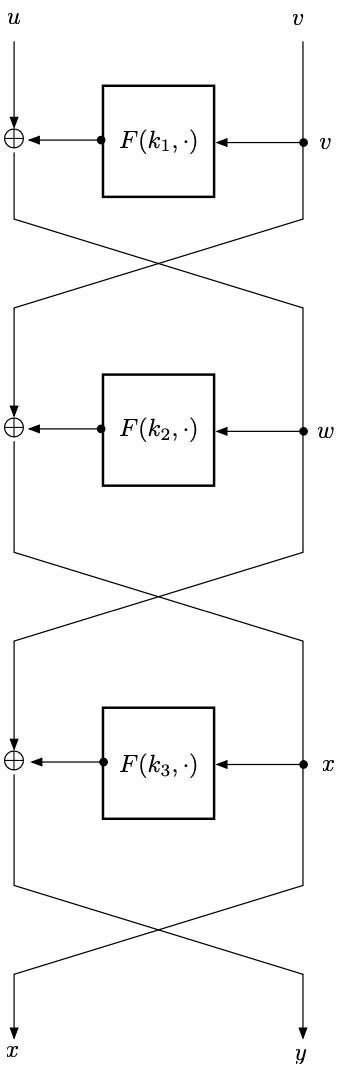
\includegraphics[width=0.28\linewidth]{figures/chapter4/fig14-a.png}}
  \quad\quad\quad\quad\quad\quad
  \subfigure[解密]{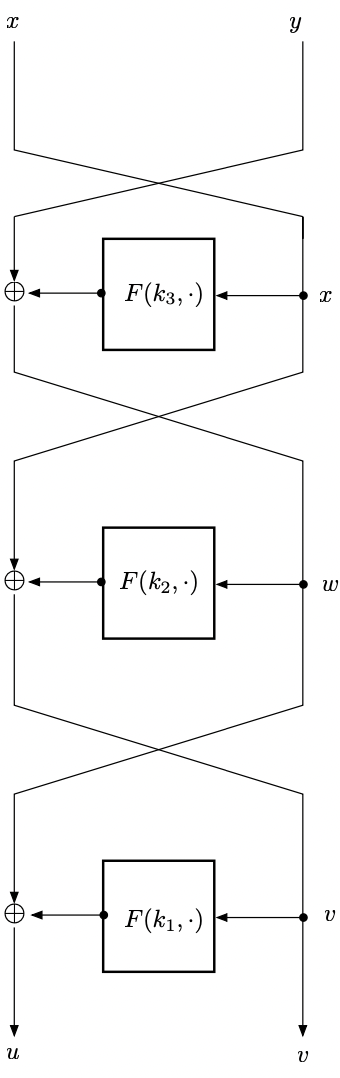
\includegraphics[width=0.28\linewidth]{figures/chapter4/fig14-b.png}}
  \caption{使用卢比-拉克福构造进行加密和解密}
  \label{fig:4-14}
\end{figure}

容易看出,$\mathcal{E}$ 是一个分组密码。可以认为算法 $E$ 由三``轮"运算组成。对于 $k\in\mathcal{K}$,我们定义``轮函数"为:
\[
\begin{aligned}
\phi_k:\quad\mathcal{X}^2 & \to \mathcal{X}^2\\
(a,b) & \mapsto (b,a\oplus F(k,b))
\end{aligned}
\]

不难看出,对于任意固定的 $k$,函数 $\phi_k$ 都是 $\mathcal{X}^2$ 上的一个置换。事实上,如果令 $\sigma(a,b):=(b,a)$,则有:
\[
\phi_k^{-1}=\sigma\circ\phi_k\circ\sigma
\]
此外,我们可以发现:
\[
E((k_1,k_2,k_3),\cdot)=\phi_{k_3}\circ\phi_{k_2}\circ\phi_{k_1} 
\]
和:
\[
D((k_1,k_2,k_3),\cdot)=\phi^{-1}_{k_1}\circ\phi^{-1}_{k_2}\circ\phi^{-1}_{k_3}=\sigma\circ\phi_{k_1}\circ\phi_{k_2}\circ\phi_{k_3}\circ\sigma
\]

\begin{theorem}
如果 $F$ 是一个安全 PRF,且 $N:=|\mathcal{X}|=2^n$ 是超多项式的,那么由 $F$ 构建的卢比-拉克福密码 $\mathcal{E}=(E,D)$ 是一个安全的分组密码。
\begin{quote}
特别地,对于每一个如攻击游戏 \ref{game:4-1} 中那样攻击 $\mathcal{E}$ 的 $Q$ 次查询BC对手 $\mathcal{A}$,都存在一个就 $F$ 进行攻击游戏 \ref{game:4-2} 的 PRF 对手 $\mathcal{B}$,其中 $\mathcal{B}$ 是围绕 $\mathcal{A}$ 的一个基本包装器,满足:
\end{quote}
\[
{\rm BC\mathsf{adv}}[\mathcal{A},\mathcal{E}]\leq3\cdot{\rm PRF\mathsf{adv}}[\mathcal{B},F]+\frac{Q^2}{N}+\frac{Q^2}{2N^2}
\]
\end{theorem}

\begin{proof}[证明思路]
根据推论 \ref{cor:4-5},由于我们假设 $N$ 是超多项式的,所以只需要证明 $\mathcal{E}$ 是一个安全 PRF 即可。因此,我们想要证明,如果对手在攻击游戏 \ref{game:4-2} 的实验 $0$ 中针对 $\mathcal{E}$ 进行游戏,挑战者的回应实际上``看起来像"完全随机的比特序列。我们可以假设对手永远不会发起两次相同的查询。此外,由于 $F$ 是一个 PRF,我们可以用真随机函数 $f_1$,$f_2$ 和 $f_3$ 来代替伪随机函数 $F(k_1,\cdot)$,$F(k_2,\cdot)$ 和 $F(k_3,\cdot)$,而对手应该很难注意到这种区别。

因此,现在给定一个查询 $(u_i,v_i)$,挑战者按如下方式计算应答 $(x_i,y_i)$:

\vspace{5pt}

\hspace*{5pt} $w_i\leftarrow u_i\oplus f_1(v_i)$\\
\hspace*{26pt} $x_i\leftarrow v_i\oplus f_2(w_i)$\\
\hspace*{26pt} $y_i\leftarrow w_i\oplus f_3(x_i)$

\vspace{5pt}

一个粗略、直观的论证是这样的。假设没有任何两个 $w_i$ 值是相同的,那么 $f_2$ 的所有输出都是随机且相互独立的。由此,我们可以论证 $x_i$ 也是随机且相互独立的。因此 $f_3$ 的输入存在相同值的概率可忽略不计。由此,我们可以得出结论,$y_i$ 们基本上都是随机且相互独立的。

因此,如果我们能证明所有的 $w_i$ 都是不同的,情况就会很好。而 $w_i$ 是由随机函数 $f_1$ 间接得到的,所以只要小心一点,确实可以论证 $w_i$ 中存在相同值的概率可忽略不计。
\end{proof}

\begin{proof}
假设 $\mathcal{A}$ 是一个有效BC对手,它对 $\mathcal{E}$ 进行攻击游戏 \ref{game:4-1} 中的攻击,并且对挑战者发起最多 $Q$ 次查询。我们想证明 ${\rm BC\mathsf{adv}}[\mathcal{A},\mathcal{E}]$ 可忽略不计。要做到这一点,我们首先要证明 ${\rm PRF\mathsf{adv}}[\mathcal{A}, E]$ 是可忽略不计的,然后基于 PRF 切换引理(即定理 \ref{theo:4-4})和 $N$ 是超多项式的假设中得出结果。

简便起见,我们用一个具备以下特性的对手 $\mathcal{A}_0$ 来代替 $\mathcal{A}$:
\begin{itemize}
	\item $\mathcal{A}_0$ 总是对其挑战者进行恰好 $Q$ 次查询;
	\item $\mathcal{A}_0$ 不会多次进行相同的查询;
	\item $\mathcal{A}_0$ 和 $\mathcal{A}$ 一样有效(更确切地说,$\mathcal{A}_0$ 是围绕 $\mathcal{A}$ 的一个基本包装器);
	\item ${\rm PRF\mathsf{adv}}[\mathcal{A}_0, E]={\rm PRF\mathsf{adv}}[\mathcal{A}, E]$。
\end{itemize}
对手 $\mathcal{A}_0$ 只是简单地运行与$\mathcal{A}$相同的协议;然而,它保留了一张查询/应答表,以避免重复查询;此外,如有必要,$\mathcal{A}_0$ 会``填充" $\mathcal{A}$ 的执行次数,以确保发起查询的次数正好是 $Q$。

该证明的总体策略如下。首先,我们将游戏 $0$ 定义为 $\mathcal{A}_0$ 与攻击游戏 \ref{game:4-2} 的实验 $0$ 的挑战者之间就 $E$ 进行的游戏。然后,我们再定义几个游戏:游戏 $1$,游戏 $2$ 和游戏 $3$。每一个游戏都是在 $\mathcal{A}_0$ 和不同的挑战者之间进行的;此外,游戏 $3$ 中的挑战者等同于攻击游戏 \ref{game:4-2} 的实验 $1$ 的挑战者。另外,对于 $j=0,\dots,3$,我们定义 $W_j$ 为 $\mathcal{A}_0$ 在游戏 $j$ 中输出 $1$ 的事件。我们将表明,对于 $j=1,\dots,3$,$|\Pr[W_j]-\Pr[W_{j-1}]|$ 的值可忽略不计,由此,我们可以得到:
\[
|\Pr[W_3]-\Pr[W_0]|={\rm PRF\mathsf{adv}}[\mathcal{A}_0, E]
\]
也是可忽略不计的。

\vspace{5pt}

\noindent
\textbf{游戏 $\mathbf{0}$}。
我们首先详细描述游戏 $0$ 中的挑战者:

\vspace{5pt}

\hspace*{5pt} 选取 $k_1,k_2,k_3\overset{\rm R}\leftarrow\mathcal{K}$\\
\hspace*{26pt} 当收到第 $i$ 个查询 $(u_i,v_i)\in\mathcal{X}^2\;\;(i=1,\dots,Q)$ 时,计算:\\
\hspace*{50pt} $w_i\leftarrow u_i\oplus F(k_1,v_i)$\\
\hspace*{50pt} $x_i\leftarrow v_i\oplus F(k_2,w_i)$\\
\hspace*{50pt} $y_i\leftarrow w_i\oplus F(k_3,x_i)$\\
\hspace*{50pt} 将 $(x_i,y_i)$ 发送给对手。

\vspace{5pt}

\noindent
回顾一下,对手 $\mathcal{A}_0$ 保证总是会发起 $Q$ 次不同的查询 $(u_1,v_1),\dots,(u_Q,v_Q)$;也就是说,$(u_i,v_i)$ \emph{作为数对}是各不相同的;所以对于 $i\neq j$,我们可能有 $u_i=u_j$ 或 $v_i=v_j$,但是两者不能同时成立。

\vspace{5pt}

\noindent
\textbf{游戏 $\mathbf{1}$}。
我们接下来打``PRF牌",即用真随机函数 $f_1$,$f_2$ 和 $f_3$ 来代替三个伪随机函数 $F(k_1,\cdot)$,$F(k_2,\cdot)$ 和 $F(k_3,\cdot)$。因此,我们在游戏 $1$ 中的挑战者运行如下:

\vspace{5pt}

\hspace*{5pt} 选取 $f_1,f_2,f_3\overset{\rm R}\leftarrow{\rm Funs}[\mathcal{X},\mathcal{X}]$\\
\hspace*{26pt} 当收到第 $i$ 个查询 $(u_i,v_i)\in\mathcal{X}^2\;\;(i=1,\dots,Q)$ 时,计算:\\
\hspace*{50pt} $w_i\leftarrow u_i\oplus f_1(v_i)$\\
\hspace*{50pt} $x_i\leftarrow v_i\oplus f_2(w_i)$\\
\hspace*{50pt} $y_i\leftarrow w_i\oplus f_3(x_i)$\\
\hspace*{50pt} 将 $(x_i,y_i)$ 发送给对手。

\vspace{5pt}

如练习 4.26 中将要讨论的,我们可以将三个伪随机函数 $F(k_1,\cdot)$,$F(k_2,\cdot)$ 和 $F(k_3,\cdot)$ 建模为一个单一的 PRF $F'$,称其为 $F$ 的 $3$ 次并行组合:PRF $F'$ 定义在 $(\mathcal{K}^3,\{1,2,3\}\times\mathcal{X},\mathcal{X})$ 上,且 $F'((k_1,k_2,k_3),(s,x)):=F(k_s,x)$。我们很容易构造一个和 $\mathcal{A}_0$ 一样有效的对手 $\mathcal{B}'$,使得:
\begin{equation}\label{eq:4-24}
|\Pr[W_1]-\Pr[W_0]|={\rm PRF\mathsf{adv}}[\mathcal{B}', F']
\end{equation}
对手 $\mathcal{B}'$ 简单地运行 $\mathcal{A}_0$,并原样输出 $\mathcal{A}_0$ 所输出的任何东西。当 $\mathcal{A}_0$ 用一个数对 $(u_i,v_i)$ 查询其挑战者时,对手 $\mathcal{B}'$ 通过计算:

\vspace{5pt}

\hspace*{5pt} $w_i\leftarrow u_i\oplus f'(1,v_i)$\\
\hspace*{26pt} $x_i\leftarrow v_i\oplus f'(2,w_i)$\\
\hspace*{26pt} $y_i\leftarrow w_i\oplus f'(3,x_i)$

\vspace{5pt}

\noindent
来得到要交给 $\mathcal{A}_0$ 的应答 $(x_i,y_i)$。这里,$f'$ 表示 $\mathcal{B}'$ 的挑战者在攻击游戏 \ref{game:4-2} 中就 $F'$ 所选择的函数。很明显,$\mathcal{B}'$ 在该攻击游戏的实验 $0$ 中以概率 $\Pr[W_0]$ 输出 $1$,而在实验 $1$ 中以概率 $\Pr[W_1]$ 输出 $1$,由此可得式 \ref{eq:4-24}。

根据练习 4.26,存在一个和 $\mathcal{B}'$ 一样有效的对手 $\mathcal{B}$,满足:
\begin{equation}\label{eq:4-25}
{\rm PRF\mathsf{adv}}[\mathcal{B}', F']= 3\cdot {\rm PRF\mathsf{adv}}[\mathcal{B}, F]
\end{equation}

\noindent
\textbf{游戏 $\mathbf{2}$}。
接下来我们做一个纯粹的概念上的改变:我们用 \ref{subsec:4-4-2} 小节中讨论的``忠实的侏儒"来实现随机函数 $f_2$ 和 $f_3$。这样做并不是为了提高效率,而是为了给我们做准备,以便之后在游戏 $3$ 中能够做出更实质性(也更易分析)的修改。我们在这个游戏中的挑战者的工作方式如下:

\vspace{5pt}

\hspace*{5pt} 选取 $f_1\overset{\rm R}\leftarrow{\rm Funs}[\mathcal{X},\mathcal{X}]$\\
\hspace*{26pt} 选取 $X_1,\dots,X_Q\overset{\rm R}\leftarrow\mathcal{X}$\\
\hspace*{26pt} 选取 $Y_1,\dots,Y_Q\overset{\rm R}\leftarrow\mathcal{X}$\\
\hspace*{26pt} 当收到第 $i$ 个查询 $(u_i,v_i)\in\mathcal{X}^2\;\;(i=1,\dots,Q)$ 时:\\
\hspace*{50pt} 计算 $w_i\leftarrow u_i\oplus f_1(v_i)$\\
\hspace*{50pt} 令 $x_i'\leftarrow X_i$;
				\framebox[\width]{~如果存在 $j<i$ 使得 $w_i=w_j$,则令 $x_i'\leftarrow x_j'$;}
				令 $x_i\leftarrow v_i\oplus x_i'$\\
\hspace*{50pt} 令 $y_i'\leftarrow Y_i$;
				\framebox[\width]{~如果存在 $j<i$ 使得 $x_i=x_j$,则令 $y_i'\leftarrow y_j'$;}
				令 $y_i\leftarrow w_i\oplus y_i'$\\
\hspace*{50pt} 将 $(x_i,y_i)$ 发送给对手。

\vspace{5pt}

\noindent
这个的想法是,$x_i'$ 的值代表 $f_2(w_i)$。默认情况下,$x_i'$ 等于随机值 $X_i$;然而,如果存在某个 $j<i$ 使得 $w_i=w_j$,上面被框住的逻辑就会覆写这个默认值。同样地,$y_i'$ 的值代表 $f_3(x_i)$。在默认情况下,$y_i'$ 等于随机值 $Y_i$,但如有必要,框住的逻辑就会覆写默认值。

由于游戏 $2$ 中的挑战者完全等同于游戏 $1$ 中的挑战者,我们有:
\begin{equation}\label{eq:4-26}
\Pr[W_2]=Pr[W_1]
\end{equation}

\noindent
\textbf{游戏 $\mathbf{3}$}。
我们现在采用``健忘的侏儒"技术,如之前在定理 \ref{theo:4-6} 的证明中介绍的那样。我们的想法是简单地消除挑战者在游戏 $2$ 中进行的的重复检查。挑战者在游戏 $3$ 中的运行流程如下:

\vspace{5pt}

\hspace*{5pt} 选取 $f_1\overset{\rm R}\leftarrow{\rm Funs}[\mathcal{X},\mathcal{X}]$\\
\hspace*{26pt} 选取 $X_1,\dots,X_Q\overset{\rm R}\leftarrow\mathcal{X}$\\
\hspace*{26pt} 选取 $Y_1,\dots,Y_Q\overset{\rm R}\leftarrow\mathcal{X}$\\
\hspace*{26pt} 当收到第 $i$ 个查询 $(u_i,v_i)\in\mathcal{X}^2\;\;(i=1,\dots,Q)$ 时:\\
\hspace*{50pt} 计算 $w_i\leftarrow u_i\oplus f_1(v_i)$\\
\hspace*{50pt} 令 $x_i'\leftarrow X_i$;令 $x_i\leftarrow v_i\oplus x_i'$\\
\hspace*{50pt} 令 $y_i'\leftarrow Y_i$;令 $y_i\leftarrow w_i\oplus y_i'$\\
\hspace*{50pt} 将 $(x_i,y_i)$ 发送给对手。

\vspace{5pt}

请注意,这一描述与游戏 $2$ 中对挑战者的描述完全相同,我们只是简单地抹去了后者中被框住的逻辑。

为了分析,我们把游戏 $2$ 和游戏 $3$ 看作是运行在相同的基础概率空间上。这个概率空间是取决于以下因素:
\begin{itemize}
	\item 对手所做的随机选择,我们用 $Coins$ 表示,以及
	\item 挑战者所做的随机选择,即 $f_1,X_1,\dots,X_Q$ 和 $Y_1,\dots,Y_Q$。
\end{itemize}
这两个游戏间的不同之处在于挑战者针对对手查询给出应答的策略。

\vspace{5pt}

\noindent
\textbf{声称$\mathbf{1}$:}
\emph{在游戏 3 中,随机变量 $Coins,f_1,x_1,y_1,\dots,x_Q,y_Q$ 是相互独立的。}为了证明这一声称,根据构造,随机变量:
\[
Coins,\quad
f_1,\quad
X_1,\dots,X_Q,\quad
Y_1,\dots,Y_Q
\]
是相互独立的。现在以 $Coins$ 和 $f_1$ 的任何固定值为条件。第一个查询 $(u_1,v_1)$ 现在是固定的,因此 $w_1$ 也是固定的;然而,在这个条件概率空间中,$X_1$ 和 $Y_1$ 仍然在 $\mathcal{X}$ 上均匀独立分布,因此 $x_1$ 和 $y_1$ 也是均匀且独立分布的。我们继续论证,以 $x_1,y_1$ 的固定值为条件(除了 $Coins$ 和 $f_1$ 的固定值之外),观察到现在 $u_2$,$v_2$ 和 $w_2$ 也是固定的,并且 $x_2$ 和 $y_2$ 是均匀独立分布的。我们应该可以清楚的看到,通过归纳法就可以证明声称 $1$ 成立。

令 $Z_1$ 表示在游戏 $3$ 中存在某个 $i\neq j$ 使得 $w_i=w_j$ 成立的事件,$Z_2$ 表示在游戏 $3$ 中存在某个 $i\neq j$ 使得 $x_i=x_j$ 成立的事件,令 $Z:=Z_1\lor Z_2$。请注意,事件 $Z$ 的定义基于游戏 $3$ 中变量 $w_i$ 和 $x_i$ 的取值。事实上,变量 $w_i$ 和 $z_i$ 在游戏 $2$ 和游戏 $3$ 中的计算方式可能不一样,所以我们在游戏 $3$ 中显式地用它们的值来定义事件 $Z$。尽管如此,我们可以直接看到,如果 $Z$ 没有发生,游戏 $2$ 和游戏 $3$ 的进程是相同的。特别是:

\vspace{5pt}

\noindent
\textbf{声称$\mathbf{2}$:}
\emph{当且仅当事件 $W_3\land\bar Z$ 发生时,事件 $W_2\land\bar Z$ 发生。}为了证明该声称,考虑事件 $Z$ 不发生的情况下,变量:
\[
Coins,\quad
f_1,\quad
X_1,\dots,X_Q,\quad
Y_1,\dots,Y_Q
\]
的任何固定值。只要说明 $\mathcal{A}_0$ 的输出在游戏 $2$ 和游戏 $3$ 中都是一样的就足够了。由于查询 $(u_1,v_1)$ 只取决于 $Coins$,我们可以看到变量 $u_1,v_1$,以及 $w_1,x_1,y_1$ 在两个游戏中都有相同的值。由于查询 $(u_2,v_2)$ 只取决于 $Coins$ 和 $(x_1,y_1)$,因此变量 $u_2,v_2$ 以及 $w_2$ 在两个游戏中都有相同的值;而由于 $Z$ 未发生,我们可知 $w_2\neq w_1$,因此变量 $x_2$ 在两个游戏中都有相同的值;同样,由于 $Z$ 未发生,因此有 $x_2\neq x_1$,所以变量 $y_2$ 在两个游戏中有相同值。以此类推,我们可以看到对于 $i=1,\dots,Q$,变量 $u_i,v_i,w_i,x_i,y_i$ 在两个游戏中都有相同值。由于 $\mathcal{A}_0$ 的输出是这些变量和 $Coins$ 的函数,所以他在两个游戏中的输出也是相同的。因此声称 $2$ 得证。

声称 $2$,连同差分引理(即定理 \ref{theo:4-7})和联合约束可以导出:
\begin{equation}\label{eq:4-27}
|\Pr[W_3]-\Pr[W_2]|\leq\Pr[Z]\leq\Pr[Z_1]+\Pr[Z_2]
\end{equation}

由于 $x_1,\dots,x_Q$ 是相互独立的(见声称$1$),显然有:
\begin{equation}\label{eq:4-28}
\Pr[Z_2]\leq\frac{Q^2}{2}\cdot\frac{1}{N}
\end{equation}
因为 $Z_2$ 是少于 ${Q^2}/{2}$ 个事件的联合,其中每个事件发生的概率为 ${1}/{N}$。

下面我们分析事件 $Z_1$。我们声称:
\begin{equation}\label{eq:4-29}
\Pr[Z_1]\leq\frac{Q^2}{2}\cdot\frac{1}{N}
\end{equation}
为了证明这一点,只需证明它是以 $Coins,x_1,y_1,\dots,x_Q,y_Q$ 的任何固定值为条件。如果这些值是固定的,那么 $u_1,v_1,\dots,u_Q,v_Q$ 也是固定的。然而,根据独立性(见声称 $1$),变量 $f_1$ 在这个条件概率空间的 ${\rm Funs}[\mathcal{X},\mathcal{X}]$ 上仍然是均匀分布的。现在,考虑任何一对固定索引 $i,j$,其中 $i\neq j$。首先假设 $v_i=v_j$,那么,由于 $\mathcal{A}_0$ 从来不会发起两次相同的查询,我们必有 $u_i\neq u_j$,而且很容易看到,对于任何 $f_1$ 的选择,都有 $w_i\neq w_j$。接下来,假设 $v_i\neq v_j$,那么 $f_1(v_i)$ 和 $f_1(v_j)$ 的值在这个条件概率空间的 $\mathcal{X}$ 上是均匀独立分布的,且在该条件概率空间上有:
\[
\Pr[f_1(v_i)\oplus f_1(v_j)=u_i\oplus u_j]=\frac{1}{N}
\]

因此,我们证明了在游戏 $3$ 中,对于任意满足 $i\neq j$ 的索引对 $i,j$,有:
\[
\Pr[w_i=w_j]\leq\frac{1}{N}
\]
那么由联合约束,就可以得到式 \ref{eq:4-29}。

作为声称 $1$ 的另一个结论,我们观察到,就 $\mathcal{E}$ 而言,游戏 $3$ 等同于攻击游戏 \ref{game:4-2} 的实验 $1$。由此,连同式 \ref{eq:4-24},\ref{eq:4-25},\ref{eq:4-26},\ref{eq:4-27},\ref{eq:4-28} 和\ref{eq:4-29},我们可以得到以下结论:
\[
{\rm PRF\mathsf{adv}}[\mathcal{A}_0,E]\leq3\cdot{\rm PRF\mathsf{adv}}[\mathcal{B},F]+\frac{Q^2}{N}
\]
最后,将定理 \ref{theo:4-4} 应用于数据分组空间大小为 $N^2$ 的密码 $\mathcal{E}$,我们就有:
\[
{\rm BC\mathsf{adv}}[\mathcal{A},\mathcal{E}]\leq3\cdot{\rm PRF\mathsf{adv}}[\mathcal{B},F]+\frac{Q^2}{N}+\frac{Q^2}{2N^2}
\]
于是该定理得证。
\end{proof}